\documentclass[onecolumn, 12pt, a4paper]{article}
\usepackage[margin=1.00in]{geometry}
\usepackage{natbib}
\bibliographystyle{icarus}
\usepackage{amsmath}
\usepackage{amssymb}
\usepackage{subcaption}
\usepackage{graphicx}
\usepackage{caption2}
\usepackage{tabu}
\usepackage{multirow}
\usepackage{siunitx}
\usepackage{amsmath}
\begin{document}



\providecommand{\e}[1]{\ensuremath{\times 10^{#1}}}

\setlength{\parskip}{0em}


\onecolumn{%}
 \centering
 \LARGE Lab 4 Report: Doppler Measurement of Solar Rotation \\[1.5em]
 %\LARGE Deformation of Mars shorelines explained by Tharsis uplift and limited true polar wander \\[1.5em]
 \large Eden Chen,
        Magdelena Allen 
        and Joseph Miller

 December 5, 2017
 
 Email: ychen3856@berkeley.edu \linebreak
 Student ID: 3032340806

\vspace{0.25in}
}
\begin{abstract}
In this lab we collected a series of solar spectrum data with a spectrometer that uses diffraction gratings to calculate the Doppler shift of Sun's rotational velocity and derived its radius and distance from Earth. We first calibrated the wavelength-pixel ratio by examining the pixel positions of Neon (Ne) light spectrum and match its emission centroids with their respective wavelengths. Six emission lines were used from the Ne spectrum to match with their known wavelengths. The ratio between the wavelength and the pixel position of our 2D spectrum images is 4.7 $\times 10^{-2} \pm 1.67 \times 10^{-3}$ pixel per one Nano meter of wavelength. Once the wavelength-pixel ratio is determined, we can then calculate the pixel shift by cross correlate 38 sets of solar transition data with its peak intensity spectrum. The average lag was calculated to be 2.25 $\times 10^{-3}$ pixels. using the lag and wavelength-pixel ratio we calculated the rotational velocity of the Sun to be 1.916 km/s and its radius to be 6.952$\times 10^5$ km. Using the Sun's angular half width of \ang{0.25} we then determined its distance from Earth to be 1.589 $\times 10^8$ km.
\end{abstract}

\section{Introduction}
One of the oldest questions is finding out the size of our Sun and its distance from us. Using modern telescope and  We can derive the Sun's distance from Earth and its radius from its rotational velocity and period. Rotational velocity can be determined by measuring the Doppler shift of the wavelength produced from a 1D solar spectrum image. The Doppler effect is the change in wavelength or frequency of a wave seen by an observer (Earth) who is moving relative to the wave source (Sun). As the Sun rotate from one direction to the other, the side where it rotates toward us will create a blue shift in wavelength and as the other side rotates away from us we will see a red shifted wave. In order to measure the wavelength shift from Sun's rotational velocity we will first need to convert the pixel position from a CCD image of Ne light to wavelength. The wavelengths of Ne light emission lines can be found from the National Institute of Standards and Technology (NIST) website. My group collected 75 sets of solar spectra with 38 of which contains the Sun's transitional intensity. By cross-correlate the 1D image of each of those transition spectra with the peak intensity spectra we can spot the difference in their pixel position. The difference will be tiny - at the magnitude of a tenth of a pixel. We can then calculate the rotational velocity of the Sun from slope of cross-correlation fit, wavelength-pixel ratio and the rest wavelength. The radius of the Sun can be deduced from the rotational speed and its period. Finally, the distance from Earth to the Sun can be measured using simple geometry. 

\section{Equipment}
The solar transition data can be obtained by using an optical fiber at the focal plane of an Newtonian telescope. The telescope is an 8-inch Celestron mounted on the NCH 541 observing platform. The data are acquired using constant declination scans at the sidereal rate. The optical fiber was connected to an Apogee $1024 \times 1024$ CCD with nominal properties listed below: \newline

\centerline{
\begin{tabu} to 0.9\textwidth { | X[l] | X[r] | }
 \hline
 Property & Value \\
 \hline
 Echelle grating groove density (1/$\sigma$)  & 80 $mm^{-1}$ \\
\hline
 Echelle blaze angle ($\theta_b$) & $\ang{64.4}$\\
 \hline
 Entrance slit width &  \SI{50}{\micro\metre}  \\
\hline
 Collimator focal length ($f_{col}$)& 100 mm\\
 \hline
 Camera focal length ($f_{cam}$)  & 135 mm \\
 \hline
 Apogee CCD pixel size & \SI{50}{\micro\metre} \\
 \hline
2 $\theta^{a}$  & $\ang{22}$ \\
 \hline
\end{tabu}}
\leavevmode
\newline

\textbf{Table 1}: Nominal spectrometer properties. where $^{a}$ is the full angle between incident and diffracted beam.

\newline

\begin{flushleft}
We also want to know the upper limit for velocity detection of our spectrometer. We can calculate this by dividing the speed of light by the spectral resolving power R, which can be found by using

\begin{equation}\label{eq:1}
R = \dfrac{2\sin{\delta}\cos{\theta}f}{\cos{\alpha} df}
\end{equation}
where $\delta$ is the Echelle blaze angle, $\theta$ is the half angle between the incident and the diffracted beam, f Collimator focal length, $\alpha$ is $\delta + \theta$ and $df$ is the entrance slit width. The spectral resolving power R is calculated to be \boxed{1.405 \times 10^4} and the upper limit for velocity detection is \boxed{21.355} km/s.
\end{flushleft}
\section{Acquiring Data}

On November 17, 2017, Elena, Joe and I collected the spectra image of a quartz-halogen lamp, a diode laser, an Ne lamp and a dark current all with the exposure time of five seconds. The CCD image of the dark current, lamps and the laser spectra was processed remotely via one of the lab's terminals located at the fifth floor of Campbell Hall, University of California, Berkeley. At the same day we collected 75 sets of solar transition spectra with the exposure time of 0.8 second under the guidance of professor James R. Graham. The total transit time of the Sun across the optical fiber slit was about 40 seconds.

\section{Data Processing}
Each 2D CCD image has the resolution of $1024 \times 1024$. In this lab my group and I collected four different spectra that includes the quartz-halogen lamp, the diode laser, the Ne lamp and the Sun. Each of these spectra have a unique sets of emission and absorption lines that can be matched with a elemental signatures. \newline
\begin{subfigure}{\linewidth}\hspace*{-.8cm}
  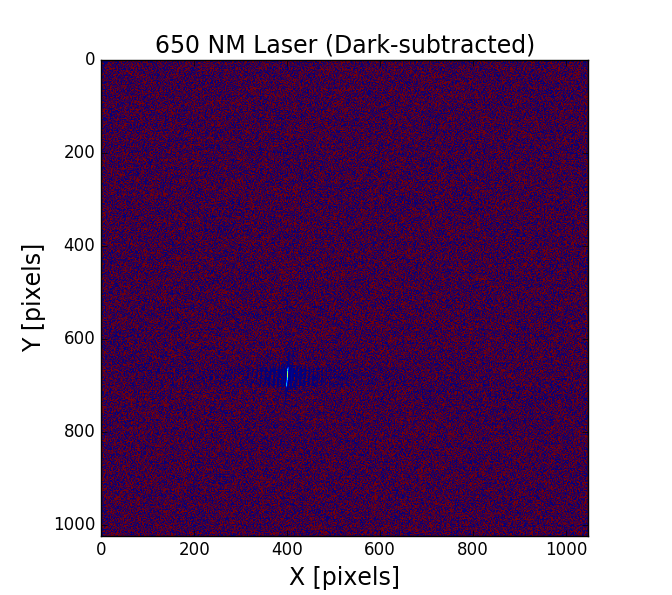
\includegraphics[width=.55\linewidth]{figure_1-11.png}
  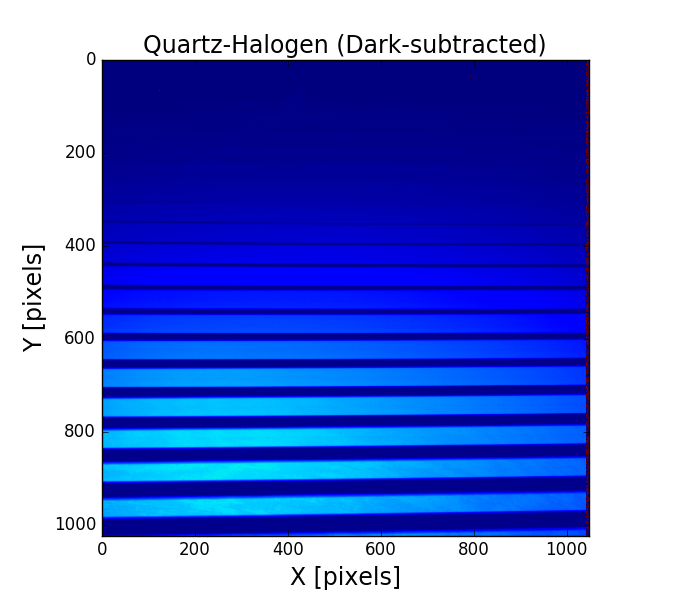
\includegraphics[width=.55\linewidth]{figure_1-12.png}
\end{subfigure}\par\medskip

\textbf{Figure 1}: Left: A 2D image of the diode laser spectra. Right: The continuum quartz-halogen lamp spectra. Both image are taken with 0.8 second exposure time.

\begin{flushleft}
For wavelength calibration I will only focus on the Ne spectra. The raw Ne spectra data was a 2D image so I will have to slice a section it to create an 1D image to calibrate the wavelength with. I chose the Echelle order of six composed of 47 rows from my Ne spectra and created Figure 1. The slice is created from row 600 to 647 on the y-axis in pixels.
\end{flushleft}
\centerline{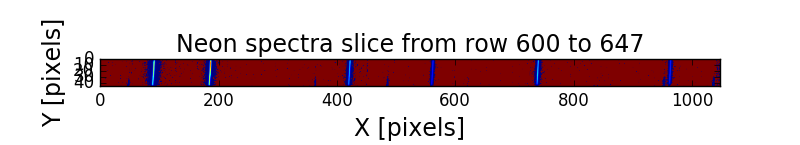
\includegraphics[width=.8\linewidth]{figure_1-2.png}}
\newline 

\textbf{Figure 2}: Sliced image of the dark-subtracted Ne spectra from row 600 to 647.\newline 

\begin{flushleft}
I then sum up the total intensity of Figure 1 vertically to create an 1D image:
\end{flushleft}
\begin{subfigure}{\linewidth}\hspace*{-.8cm}
  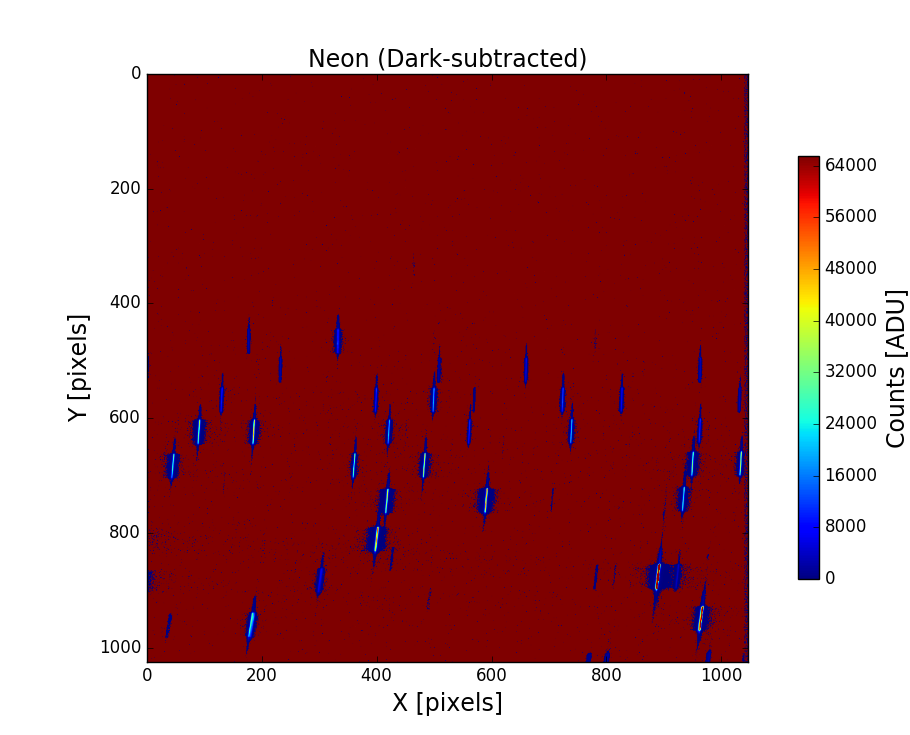
\includegraphics[width=.55\linewidth]{figure_1.png}
  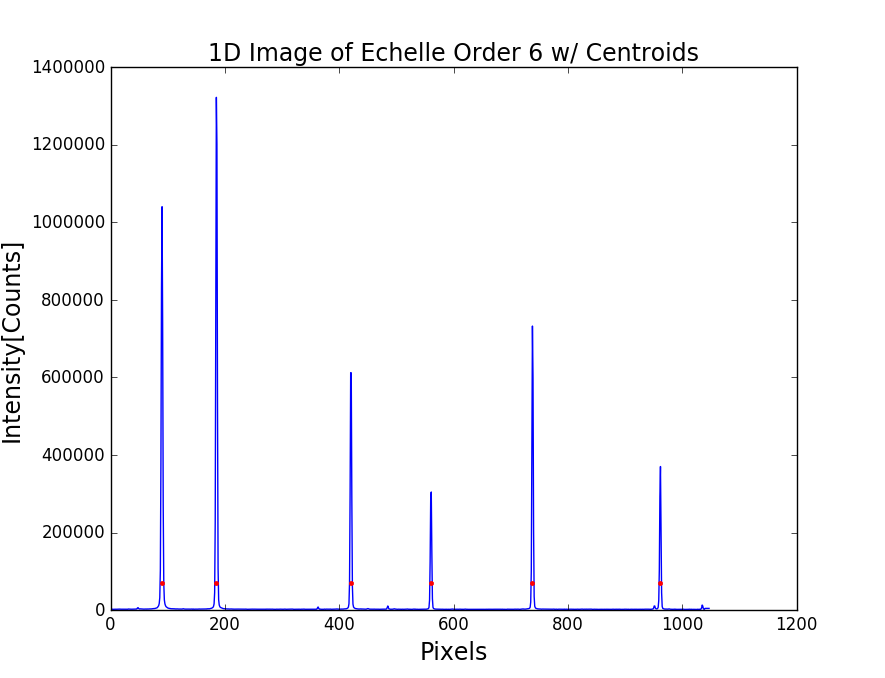
\includegraphics[width=.55\linewidth]{figure_1-1.png}
\end{subfigure}\par\medskip

\textbf{Figure 3}: Left: The 2D CCD image of the dark-subtracted Ne spectra. Right: The 1D plot of the Ne spectra created from summing up the intensity in Figure 1 vertically. \newline

\begin{flushleft}
Six centroids from each emission peaks in pixel number from Figure 2 can be matched with their known wavelength position from the National Institudte of Standard and Technology (NIST). The respective wavelength for each of the centroid positions in Figure 2 are:
\end{flushleft}
\newline 

\hspace*{-.6cm}\begin{tabular}{ |p{2cm}|p{1.8cm}|p{1.8cm}|p{1.8cm}|p{1.8cm}|p{1.8cm}|p{1.8cm}| }

 \hline
  & 1st Match & 2nd Match & 3rd Match & 4th Match & 5th Match & 6th Match \\
 \hline
 Centroids (Pixels) & 89.717 & 184.988 & 420.202 & 560.251 & 737.997 & 961.691\\
 \hline
 Wavelength (nm) & 609.616 & 614.316 & 626.649 & 633.443 & 640.225 & 650.654 \\
 \hline
\end{tabular}
\leavevmode
\newline

\centerline{\textbf{Table 2}: Wavelength and pixel position match from a slice of the Ne spectra.}

\newline
\section{Wavelength Calibration}
\begin{flushleft}
We can now match the pixel positions and their respective wavelengths using a linear fit and its slope would be the wavelength-pixel ratio.
\end{flushleft}

\centerline{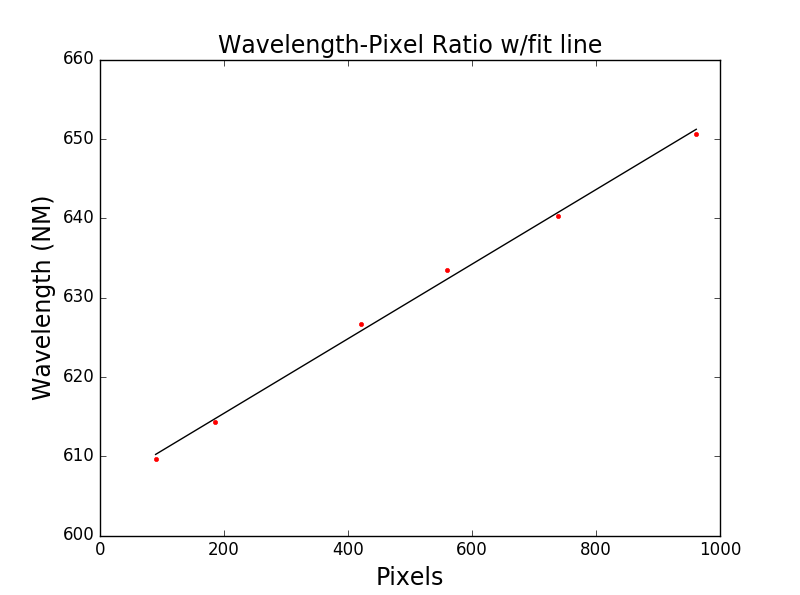
\includegraphics[scale=0.5]{figure_1-3.png}}

\textbf{Figure 4}: The wavelength-pixel ratio plot with a fit line showing a linear behavior with a slope of m = 0.047.

\begin{flushleft}
According to the slope in Figure 3, one Nano-meter of wavelength is the equivalent of \boxed{4.7\times10^{-2} \pm 0.00167} pixel in our CCD images.
\end{flushleft}
\section{Solar Transition}

In this lab my group and I collected 75 sets of solar spectra with each CCD image roughly 4 seconds apart. We can plot a 2D image of the spectra taken directly at Sun's center. We know this by examine the intensity of each data sets and the most intense one would be the Sun's center.

\centerline{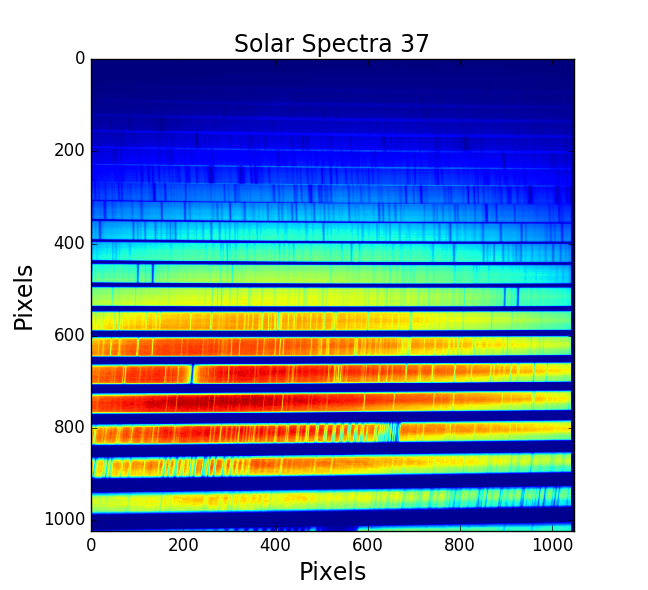
\includegraphics[width=.55\linewidth]{figure_1-4.png}} \newline

\textbf{Figure 5}: A 2D image of the most intense solar spectra. Echelle order of three to six are the most intense. This spectra being the most intense image tells us that this image was directly at the Sun's center.

\begin{flushleft}
Only 38 sets of spectra contains the Sun's spectra each with different amount of average intensity. We can the average intensity in each spectra together and create a transition plot of the Sun's flux. 
\end{flushleft}

\centerline{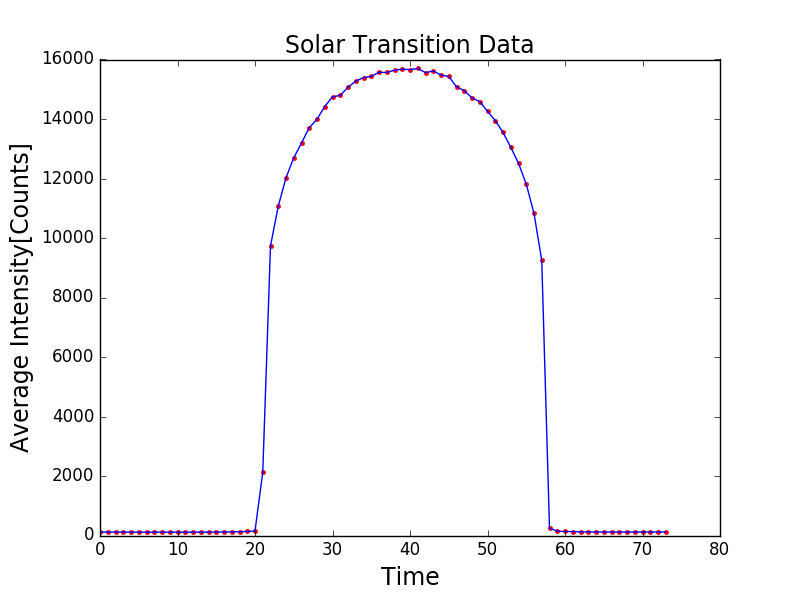
\includegraphics[width=.55\linewidth]{figure_1-5.png}}\newline

\textbf{Figure 6}: 75 sets of solar transition data plotted against their intensities. As we can see that spectra 37 is the most intense spectra that located at the center of the transition curve. Only the 22st to 58th spectra contains the transition data. Each image is taken 4 seconds apart, so the total transition time of the Sun is 38 $\times$ 4 = 152 seconds. \newline

In Figure 6 I also plotted the Eddington approximation fit to better visualize the limb darkening effect. In order to find the the shift in pixel between each transitioning spectra we will have to slice each image and compare their 1D images. We again create a slice from a 2D image of spectra 37 using row 660 to 703. This slice is using the fifth Echelle order from spectra 37.  \newline

\centerline{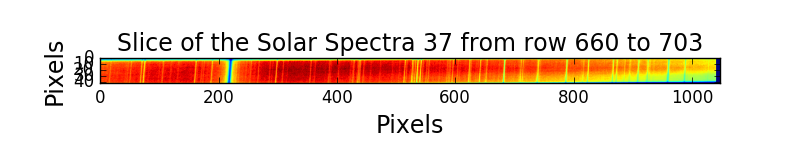
\includegraphics[width=.65\linewidth]{figure_1-6.png}}\newline

\textbf{Figure 7}: A slice of the solar spectra 37 using the fifth Echelle order. The slice is created from row 660 to 703 in the y-axis.
\begin{flushleft}
We can now create an 1D image from Figure 6 by summing up its intensity vertically: \newline
\end{flushleft}
\centerline{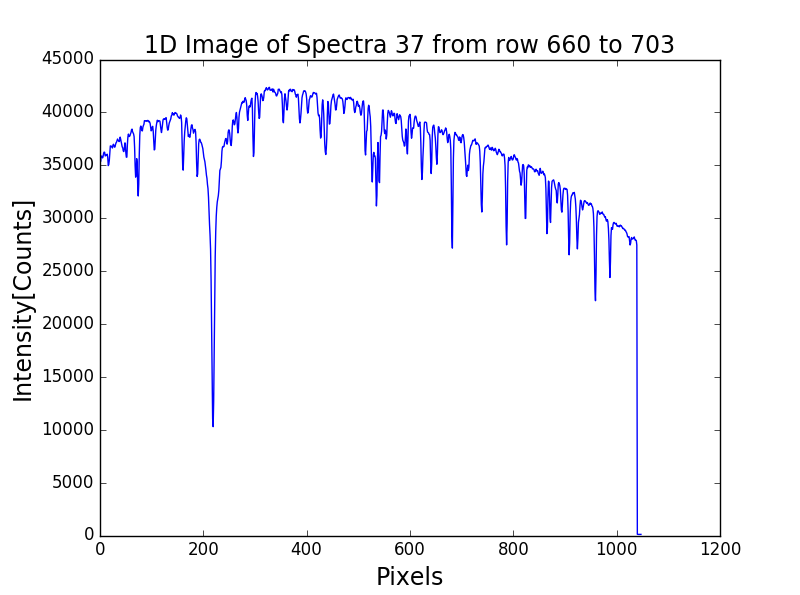
\includegraphics[width=.55\linewidth]{figure_1-7.png}}\newline

\textbf{Figure 8}: The 1D image of the solar transition spectra 37 composed from row 660 to 703.

\section{Doppler Shift Measurement}
By plotting two different spectra from different time together we can physically observe a shift in pixel. I specifically chose spectra 38 to compare with spectra 37 because choosing two spectra with a big difference in time would create a significant shift in intensity and makes it difficult to see the shift in pixels. \newline

\begin{subfigure}{\linewidth}\hspace*{-1.5cm}
  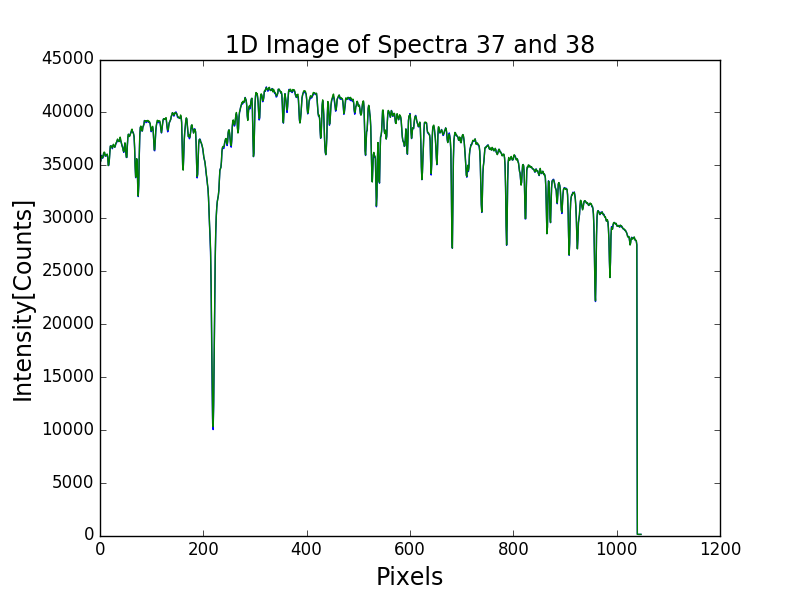
\includegraphics[scale=.45]{figure_1-8.png}
  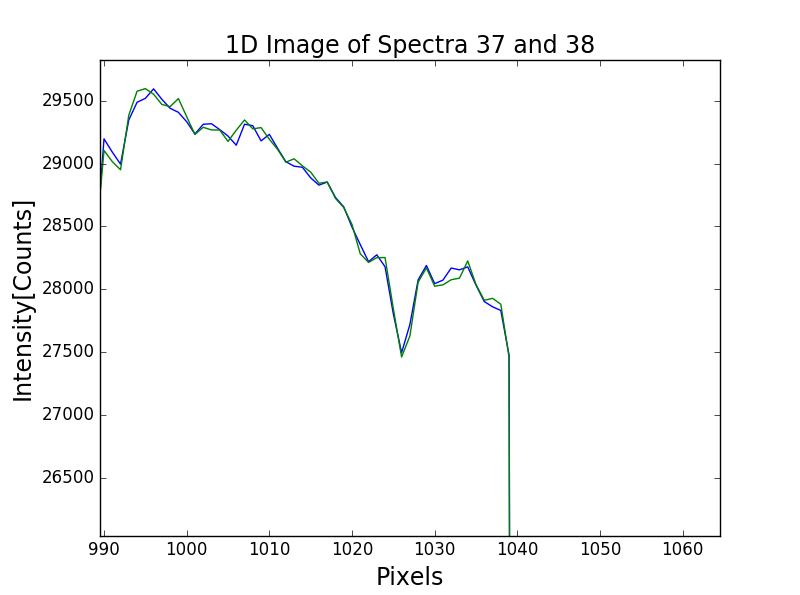
\includegraphics[scale=.45]{figure_1-9.png}
\end{subfigure}\par\medskip

\textbf{Figure 9}: Left: Compared image between spectra 37 (green) and 38 (blue). Right: Zoomed in version of the left. We can clearly observe a small shift in pixel position toward the left. The shift is very small, on the magnitude of a hundredth of a pixel. \newline

In order to measurement the velocity shift between each spectra from the entire solar transition we will need to do a cross-correlation between two spectral lines from different images. I chose to compare all the solar images from spectra 22 to 58 with spectra 37. Having the central spectra be the fixed reference frame to compare all other spectra with allow us to better identify each shift corresponds to the maximum shift.\newline

\centerline{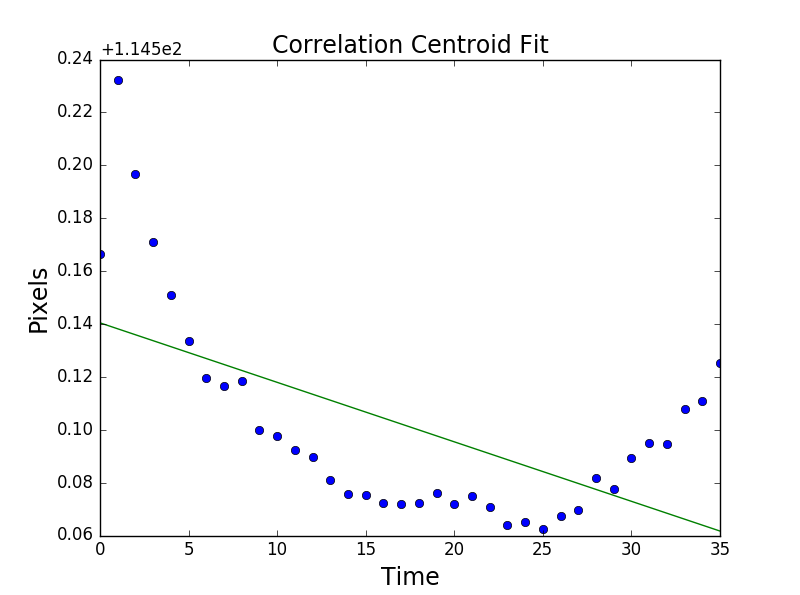
\includegraphics[scale =0.45]{figure_1-10.png}}\newline

\textbf{Figure 10}: The pixel position of a single centroid from each solar transition spectra (Spectra 21 - 59) compared with the central spectra (Spectra 37). \newline

The linear fit slope in Figure 10 is measured to be \boxed{-2.250 \times 10^{-3}}. This means that there is an average pixel shift of $2.250 \times 10^{-3}$ pixel between each transition spectra with the central solar spectra. We can see that in Figure 10 the pixel shift is at the highest during the beginning of the Sun's transition across the optical slit.
 
\section{Sun's Rotational Velocity}

The rotational velocity of the Sun can be calculated from deriving the Doppler shift equation with :

\begin{equation}\label{eq:2}
\delta \lambda = \dfrac{v}{c} \lambda_0
\end{equation}
Where $\delta \lambda$ is the spectral resolution, v is the rotational velocity (m/s), c is the speed of light (m/s) and $\lambda_0$ is the rest wavelength (NM). We also know the spectral resolution is also equal to:

\begin{equation}\label{eq:3}
\delta \lambda = m \Delta t \dfrac{d\lambda}{dp}
\end{equation}
\begin{flushleft}
Where m is the average pixel shift between each transition spectra with the central solar spectra, $\Delta t$ is the average time difference between each solar transition spectra in seconds, $\frac{d\lambda}{dp}$ is the wavelength-pixel ratio calculated from Figure 4. Combining equation 2 and 3 we get:
\end{flushleft}
\begin{equation}\label{eq:4}
v_{rot} = m \Delta t \dfrac{d\lambda}{dp} \dfrac{1}{\lambda_0} c
\end{equation}
\begin{flushleft}
 The rest wavelength  $\lambda_0$ is derived from the pixel in the middle of the spectrum (pixel # 512). Using the wavelength-pixel ratio from wavelength calibration section we can determine the rest wavelength to be 632.187 nm. By using the central pixel to calculate the rest wavelength will induce a small error, but an error that cancels across the spectrum we are using. We can plug in all the calculated variables from the following table: \newline
\end{flushleft}
\newline

\hspace*{1cm}\begin{tabular}{ |p{2.7cm}|p{1.6cm}|p{2.5cm}|p{2cm}|p{2cm}| }
 \hline
  m (Pixels/s) & $\Delta t$ (s) & $\frac{d\lambda}{dp}$ (nm/s) & $\lambda_0$ (nm) & c (m/s) \\
 \hline
 $2.250 \times 10^{-3}$ & 1.42 & $4.70 \times 10^{-2}$ & 632.187 & $3 \times 10^8$ \\
 \hline
\end{tabular}
\leavevmode
\newline 
\newline

\textbf{Table 3}: All the variables needed in equation 4 calculated from previous sections that will be used to calculate the rotational velocity of the Sun.

\begin{flushleft}
By plugging all the variables from Table 3 into equation 4 we calculated the rotational velocity of the Sun to be \boxed{1.907} km/s.
\end{flushleft}

\section{Solar Radius}

Once we have determined the rotational velocity of the Sun we can now measure the radius of the Sun. The solar radius can be calculated by comparing the observed solar rotational period, $T_{rot}$ with the rotational velocity of the Sun's surface. The rotational velocity $v_{rot}$ can be expressed as 

\begin{equation}\label{eq:5}
v_{rot} = \dfrac{2\pi R_{\odot}}{T_{rot}}
\end{equation}

hence,

\begin{equation}\label{eq:6}
R_{\odot} = \dfrac{1}{2\pi} v_{rot} T_{rot}
\end{equation}
\begin{flushleft}
Where $v_{rot}$ is the solar surface rotational velocity (km/s) and $T_{rot}$ is the rotation period (s). The rotation period can be established by observing the motion of sun spots. $T_{rot}$ have been measured to be 26.4 days or \boxed{2.26 \times 10^6} seconds. By plugging in $v_{rot}$ and  $T_{rot}$ we calculated the solar radius $R_{\odot}$ to be \boxed{6.919 \times 10^5} km.
\end{flushleft}

\section{The Earth-Sun Distance}
Finally, we can calculate the Earth-Sun distance knowing the angular diameter of the sun $\theta_{\odot}$ and its radius $R_{\odot}$. The angular diameter of the Sun is roughly the same as that of the Moon, at $\theta_{\odot}$ = \boxed{\ang{0.5}} or $8.727 \times 10^{-3}$ rad. To compensate the fact that we are only using half of the solar diameter we will have the halve the angular diameter of the Sun $\frac{\theta_{\odot}}{2}$. The Earth-Sun distance can then be expressed as:

\begin{equation}\label{eq:6}
d = \dfrac{R_{\odot}}{\arctan{(\frac{\theta_{\odot}}{2})}}
\end{equation}

\begin{flushleft}
Where $R_{\odot}$ is the solar radius in km and $\frac{\theta_{\odot}}{2}$ is the angular radius of the Sun in radiance. The Earth-Sun distance is calculated to be $1.582 \times 10^8$ km or \boxed{1.057} AU.
\end{flushleft}

\section{Discussion}
The Doppler Effect is a powerful phenomenon to exploit when measuring the motion and the distance of stellar objects. It can be used to measure the radial velocity shift of a star caused by its neighboring planets or stars, this method is called Doppler spectroscopy. Doppler spectroscopy is an indirect method for finding exoplanets and brown dwarfs from measuring the radial-velocity shift of the planet's parent star via observation of Doppler shifts in their light spectrum. With enough precision and technology, this method could be used to detect much smaller objects like dwarf planets or even asteroids around an extrasolar system. Cosmological application could include the detection of fast rotating neutron stars or black holes. 

\section{Conclusion}
In this lab my group and I collected 75 sets of solar transition data to measure the average Doppler shift in pixel between each spectra. We calibrated the wavelength-pixel ratio by finding the slope of the fit line between pixel centroids and their respective wavelengths. The slope is measured to be \boxed{4.7 \times 10^{-2}} (pixel/nm). The average pixel shift was measured by cross-correlating the spectra of the center of the Sun with the rest of the transition spectra. The average pixel shift was calculated to be \boxed{2.250 \times 10^{-3}} pixel between each CCD image. Once we know how much pixel shift occurred between each image, we can derive the Sun's rotational velocity $v_{rot}$. The rotational velocity was calculated to be \boxed{v_{rot} = 1.907} km/s using equation 4. By combining the Sun's rotational velocity and period we measured the solar radius $R_{\odot}$ to be \boxed{6.919 \times 10^5} km. Finally, we calculated the Earth-Sun distance d using the solar radius $R_{\odot}$ with equation 7 and calculated it to be \boxed{1.582 \times 10^8} km.

\begin{thebibliography}{9}

\bibitem{Graham} Graham, J. R. (2017). The Solar Spectrometer.\\

\\\texttt{https://docs.google.com/document/d/1EK-j6BjRmdz0xsC$_$fzrRzIc3zjZSjwyHyQoIEbkSgS4
\\ /edit}

\bibitem{Graham} Graham, J. R. (2015). Solar Observing\\

\\\texttt{https://drive.google.com/file/d/0B40Ynk22SiBpX2dvRFZzbEdZQmc/view}

\bibitem{Graham} Graham, J. R. (2017). Solar Coordinates & Radial Velocity.\\

\\\texttt{https://drive.google.com/file/d/0B40Ynk22SiBpelhaNDhlN19RQlU/view}

\bibitem{Graham} Domagalski, S. R. (2017). Cross-Correlating Spectra Lines.\\

\\\texttt{http://w.astro.berkeley.edu/~domagalski/ay120/crosscorr.pdf}
\end{thebibliography}

\end{document}